\documentclass[convert={density=300,outext=.png}]{standalone}
\usepackage{tikz}

\begin{document}
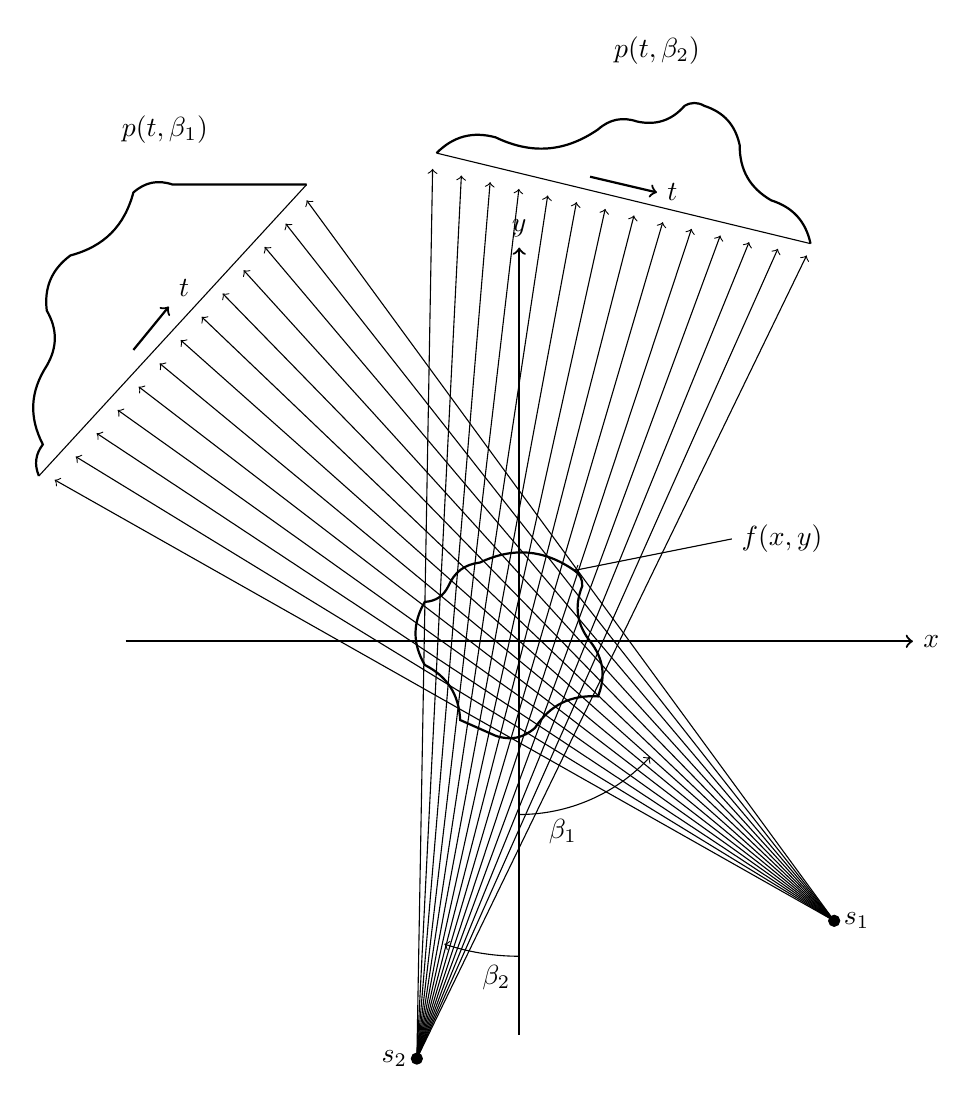
\begin{tikzpicture}[axis/.style={thick,->}]
    \draw[axis] (-5, 0) -- (5, 0) node [right] {$x$};
    \draw[axis] (0, -5) -- (0, 5) node [above] {$y$};

    % Objekt
    \draw[thick] (0.9, 0) to [bend left] (0.8, 0.7) to [bend right] (0.7, 0.9) to [bend right] (-0.5, 1)
                          to [bend right] (-0.9, 0.7) to [bend left] (-1.2, 0.5)
                          to [bend right] (-1.2, -0.3) to [bend left] (-0.75, -1) to (-0.3, -1.2)
                          to [bend right] (0.2, -1.1) to [bend left] (1, -0.7) to [bend right] (0.9, 0.0);
    \draw[->] (2.7, 1.3) -- (0.7, 0.9) node [pos=0, right] {$f(x, y)$};

    % Quellen
    \coordinate (s1) at (4, -3.55);
    \coordinate (s2) at (-1.3, -5.3);
    \draw[fill=black] (s1) circle (2pt) node [right] {$s_1$};
    \draw[fill=black] (s2) circle (2pt) node [left] {$s_2$};

    % Detektor 1
    \draw (-6.1, 2.1) -- (-2.7, 5.8);
    \draw[axis] (-4.9, 3.7) -- (-4.45 , 4.25) node [above right] {$t$};
    \draw[thick] (-6.1, 2.1) to [bend left] (-6.05, 2.5) to [bend left] (-6, 3.5) to [bend right] (-6, 4.2)
                             to [bend left] (-5.7, 4.9) to [bend right] (-4.9, 5.7) to [bend left] (-4.4, 5.8)
                             to (-2.7, 5.8);
    \node at (-4.5, 6.5) {$p(t, \beta_1)$};

    % Strahlen zu Detektor 1
    \foreach \w in {0,...,12}
        \draw[->] (s1) -- (-5.9 + \w * 0.266666666666, 2.05 + \w * 0.295833333333333);

    % Detektor 2
    \draw (-1.05, 6.2) -- (3.7, 5.05);
    \draw[axis] (0.9, 5.9) -- (1.75, 5.7) node [right] {$t$};
    \draw[thick] (-1.05, 6.2) to [bend left] (-0.3, 6.4) to [bend right] (1, 6.5) to [bend left] (1.5, 6.6)
                              to [bend right] (2.1, 6.8) to [bend left] (2.35, 6.8) to [bend left] (2.8, 6.3)
                              to [bend right] (3.2, 5.6) to [bend left] (3.7, 5.05);
    \node at(1.75, 7.5) {$p(t, \beta_2)$};

    % Strahlen zu Detektor 2
    \foreach \w in {0,...,13}
        \draw[->] (s2) -- (-1.1 + \w * 0.36538415384, 6 - \w * 0.084615384);

    % Winkel
    \draw[->] (0, -2.2) arc (270:317.5:22.5mm) node[pos=0.3,below] {$\beta_1$};
    \draw[->] (0, -4) arc (270:251.5:30mm) node[pos=0.3,below] {$\beta_2$};
\end{tikzpicture}
\end{document}
